\documentclass[10pt,twoside]{article}
\usepackage[utf8]{inputenc}
\usepackage{amsmath}
\usepackage{amsfonts}
\usepackage{amssymb}
\usepackage[spanish,es-noshorthands]{babel}
\usepackage[T1]{fontenc}
\usepackage{lmodern}
\usepackage{graphicx,hyperref}
\usepackage{tikz,pgf}
\usepackage{multicol}
\usepackage{subfig}
\usepackage[papersize={6.5in,8.5in},width=5.75in,height=7.3in]{geometry}

\author{Comité sindical\thanks{Colegio Arborizadora Baja I.E.D.}}
%\title{
%}
\date{}
\begin{document}
\begin{minipage}{.2\textwidth}

\includegraphics[height=1.55cm]{Images/logo-colegio.png}\end{minipage}
\begin{minipage}{.75\textwidth}
\begin{center}
\textbf{\large Colegio Arborizadora Baja I.E.D. (J.M.)}\\
\textbf{\large Guía Educativa para Estudiantes Ciclos 4 y 5}\\
\end{center}
\end{minipage}\hfill
\vspace*{-10pt}
\begin{center}
\large Comité sindical
\end{center}
\vspace*{-10pt}
%\maketitle
\subsection*{Logros}
\begin{itemize}
\item Que los estudiantes identifiquen algunos de los problemas sociales, económicos y políticos  que han afectado al Sector Educativo hasta hoy.
\item Construir en los estudiantes un pensamiento crítico frente a las diferentes problemáticas educativas y lograr que se involucren en la Defensa de la Educación Pública.
\end{itemize}
\section*{¿Por qué necesitamos hacer un alto en el camino?}
Para que un país pueda superar el atraso y realmente llegue a ser un país educado (no necesariamente el mejor) se necesita que la educación se garantice para todos los ciudadanos sin distinción de raza, credo o filiación política, desde la primera infancia hasta la universidad. Actualmente en nuestro país la educación no se garantiza para todos y todas. Las cifras son contundentes al respecto, pues Colombia es uno de los países de latinoamérica que menos invierte en educación y un enorme sector de la población no logra acceder a todos los niveles educativos, empezando con la primera infancia donde un gran porcentaje de los niños no está en la escuela y terminando con la universidad dónde un porcentaje muy pequeño de los egresados logra entrar a la universidad.

En esa perspectiva, nuestra federación de Trabajadores de la Educación Fecode ha presentado desde el 28 de febrero un pliego de peticiones al gobierno nacional, dónde resaltan los siguientes puntos:
\begin{enumerate}
\item Política educativa:
\begin{enumerate}
\item Se le solicita al gobierno nacional garantizar la gratuidad y obligatoriedad de la educación desde los tres grados de preescolar hasta la educación media y complementaria.
\item  b) Incrementar la inversión en educación hasta que ésta inversión llegue al 7.5\% del PIB (\textit{Colombia invertía en el 2013 el 4.9\% del PIB}). Colombia es uno de los países aspirante a ser miembro de la Organización para la Cooperación y el Desarrollo Económico (\textbf{OCDE}) que menos invierte en educación. Según cifras de la misma OCDE para el año 2015, Colombia invirtió \$3291 dólares por habitante en educación, mientras que por ejemplo Chile invirtió \$5.231 por habitante en el mismo año y si nos comparamos con  Luxemburgo, que invirtió \$17.481 dólares por habitante en el año, Luxemburgo invierte en un habitante, lo que Colombia invierte en más de 5 colombianos. Así Colombia ocupa el segundo deshonroso lugar en el ranking de los países de la \textit{OCDE} que menos invierte en educación, y así, queremos ser el país más educado en el año 2025.
\begin{center}
\textbf{Inversión en educación por habitante al año en dólares}
\begin{tabular}{|l|r@{.}l|}
\hline 
\textbf{País} & \textbf{Inversión} \\ 
\hline 
Indonesia & \$1&397 \\ 
\hline 
Colombia & \$3&291 \\ 
\hline 
Brazil & \$3&441 \\ 
\hline 
Mexico & \$3&509 \\ 
\hline 
Chile & \$5&235 \\ 
\hline 
\ldots & &\ldots \\ 
\hline 
Noruega & \$15&494 \\ 
\hline 
Suiza & \$15&497 \\ 
\hline 
Luxemburgo & \$17&485 \\ 
\hline 
\end{tabular} 
\end{center}
\item Reformar el Sistema General de Participación SGP, para garantizar los recursos para la educación pública. En el 2001 mediante el acto legislativo 01, se reformó la manera en que el estado distribuía los recursos a las regiones (\emph{se derogó el Situado fiscal y se creó el SGP}) y con ésto se produjo una reducción de los recursos que se destinarían a educación, salud y saneamiento básico. Luego en el 2007 hubo otra reforma que redujo significativamente los recursos nuevamente para educación, salud y saneamiento básico. Se calcula que el sector educativo dejó de percibir recursos por 
\item Reactivar y poner en marcha las JUME, JUDI, JUDE y JUNE, la
convocatoria de 1os foros educativos de manera concertada con
Fecode y 1os sindicatos filiales y la pluralidad pedagógica. Se supone que éstas juntas están en la ley y actualmente no funcionan. Desde estos espacios es que se deben plantear las necesidades educativas al interior de los municipios y las diferentes entidades territoriales.
\item Garantizar la proyección de la escuela como territorio de paz
\item Revisar las relaciones técnicas maestro-alumnos-aula de clase,
teniendo en cuenta las realidades de 10s contextos en
correspondencia con las recomendaciones de la ONU.
\end{enumerate}
\end{enumerate}
\subsection*{Actividad}
\begin{enumerate}
\item Ver el vídeo ¿cómo viven los niños las pruebas estandarizadas (Los Simpsons) y contestar al respecto:
\begin{enumerate}
\item Creen Ud que el resultado de una prueba estandarizada refleja la calidad de la educación de un estudiante, de un grupo de estudiantes o de un plantel educativo?
\item ¿Cree justo que los planteles educativos deban recibir recursos de acuerdo a sus resultados en las pruebas externas? Si son buenos los resultados más recursos y si no son tan buenos entonces menos recursos? ¿No debiera procederse al contrario y fortalecer el presupuesto para aquellas instituciones que se encuentren rezagadas?
\end{enumerate}
\item ¿Cómo garantizará el gobierno la universalidad de la educación cuando por ninguna parte habla de aumentar el presupuesto para educación? ¿Cómo garantizará el gobierno el acceso a la educación a los ciudadanos que no tienen recursos para acceder a la educación privada?
\item Según estudios, para poder implementar la jornada única, deberían construirse 3000 nuevos colegios. Si el gobierno planea construir solamente unos pocos, ¿cómo cree Ud que podrá implementar la jornada única?
\item Si no se construyen más colegios y el número de estudiantes se mantiene constante o incluso podría aumentar, ¿que pasará con las jornadas tarde?
\item Relación técnica de estudiante/docente según la norma NTC 4595 de 1999 del ICONTEC que a su vez establece:
\begin{center}
\begin{tabular}{|c|p{3.5cm}|c|}
\hline 
Ambiente & \# máximo de estudiantes/maestro & Área ($m^{2}$/estudiante \\ 
\hline 
Prejardín (3-4 años) & \hspace*{1cm}15 & 2,00 \\ 
Jardín (4-5 años) & \hspace*{1cm}20 & 2,00 \\ 
Transición (5-6 años) & \hspace*{1cm}30 & 2,00 \\ 
Básica y media (6-16 años) & \hspace*{1cm}40 & 1,65 a 1,80 \\ 
Especial & \hspace*{1cm}12 & 1,85 \\ \hline
\end{tabular} 
\end{center}
Cree Ud que aquí en nuestra institución se cumple con éstos parámetros en cuanto a número de estudiantes y espacio que debe tener cada estudiante en el aula?
\item Si el gobierno se comprometió a aumentar el porcentaje del PIB al 7.5\% para inversión en educación y éste no aparece en el PND, ¿cree Ud que se cumplirá lo prometido?
\begin{minipage}{.4\textwidth}
\begin{center}
\begin{tabular}{|c|c|}
\hline 
País & \% del PIB~\footnote{Datos promedio según la Comisión Económica para América Latina y el Caribe (CEPAL) en el período 2010-2013} \\ 
\hline 
Bolivia & 5.69 \\ 
\hline 
Colombia & 3.16 \\ 
\hline 
Cuba & 16.53 \\ 
\hline 
Ecuador & 4.66 \\ 
\hline 
Venezuela & 5.64 \\ 
\hline 
\end{tabular}
\end{center}
\end{minipage}
\begin{minipage}{.55\textwidth}
\item Según los datos de la tabla anterior, ¿cuál será el país que tiene un mejor sistema educativo? ¿cuál el peor? ¿Cree Ud que la inversión que hace un país está directamente relacionada con el nivel de su sistema educativo?
\end{minipage}
\item ¿Cree Ud justas las reclamaciones y peticiones que hace el magisterio colombiano?
\item Redacte una frase con la cual Ud manifiesta defender la educación pública de nuestro país.
\item De tarea en casa consultar que es el PIB (Producto Interno Bruto).
\item ¿Que piensa acerca de las siguientes dos caricaturas?

\begin{minipage}{.45\textwidth}

\includegraphics[scale=.325]{Images/quino-1.png} 
\end{minipage}\hfill
\begin{minipage}{.45\textwidth}
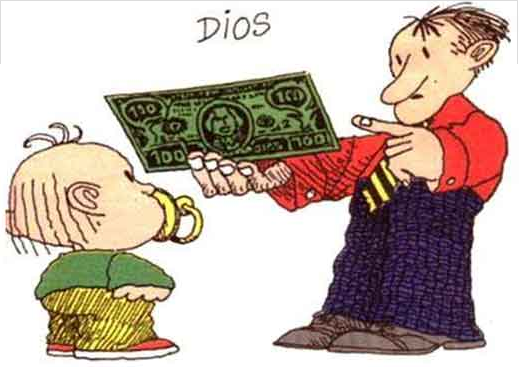
\includegraphics[scale=.325]{Images/quino-2.png} 
\end{minipage}
\item Haga una caricatura o dos acerca de la educación.
\end{enumerate}
\end{document}
